\chapter{Results}

\section{Torque estimation}
As shown in Figures 
\begin{figure}[htbp]
  \centering
  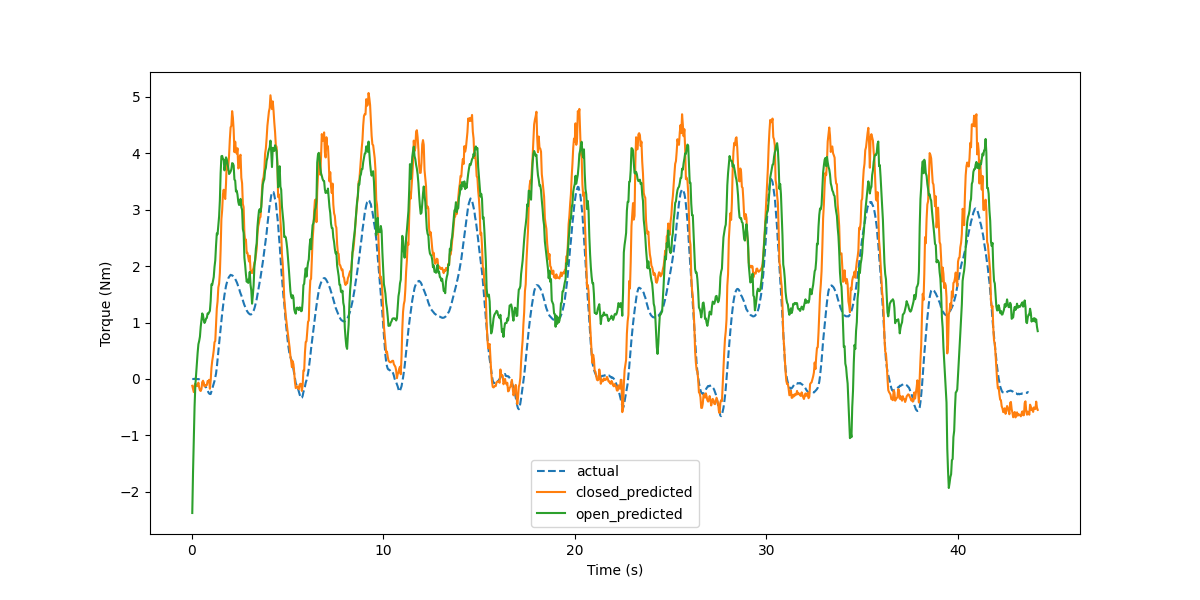
\includegraphics[width=\textwidth]{open_vs_closed_0g.png}
  \caption{}
  \label{fig:ovc0g}
\end{figure}
\begin{figure}[htbp]
  \centering
  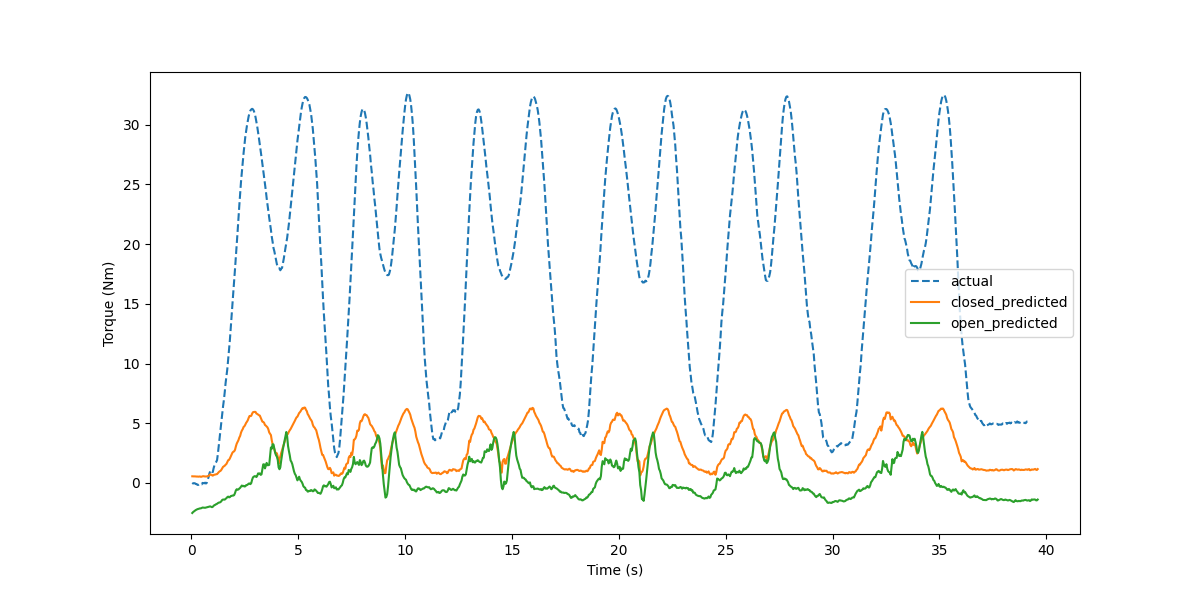
\includegraphics[width=\textwidth]{open_vs_closed_10kg.png}
  \caption{Experimental setup}
  \label{fig:ovc0g}
\end{figure}
\begin{figure}[htbp]
  \centering
  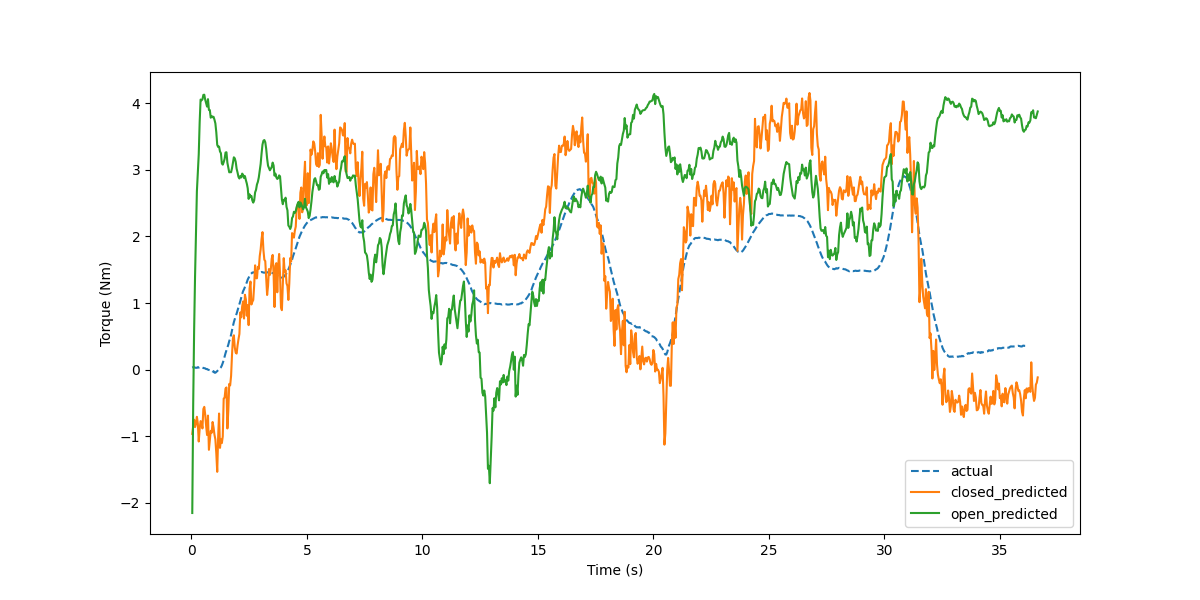
\includegraphics[width=\textwidth]{open_vs_closed_0g_stops.png}
  \caption{Experimental setup}
  \label{fig:ovc0g}
\end{figure}
\begin{figure}[htbp]
  \centering
  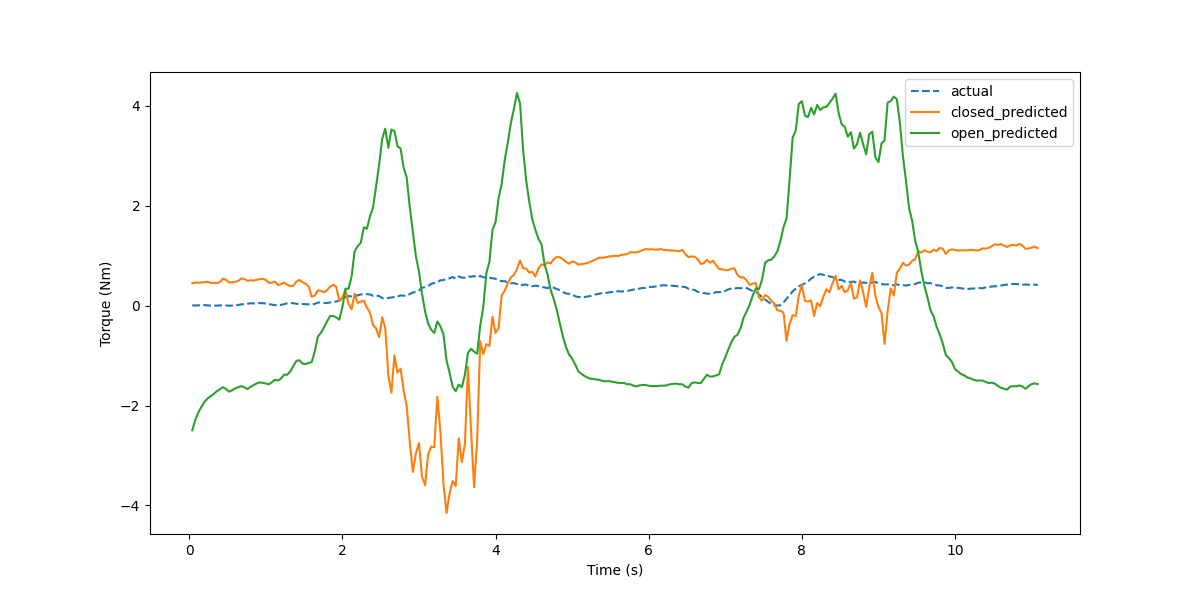
\includegraphics[width=\textwidth]{open_vs_closed_too_heavy.png}
  \caption{}
  \label{fig:ovc0g}
\end{figure}
\FloatBarrier

\section{Experimental setup}
The experimental setup is illustrated in Figure \ref{fig:setup}. The motor driver 
is first connected to the PC via USB, then the motor is securely tightened to the 
table surface and connected to the driver. The power supply is then also connected 
to the driver via a twisted pair power cable. Finally, the rope is tightened to 
prepare the system for testing.  

\begin{figure}[htbp]
  \centering
  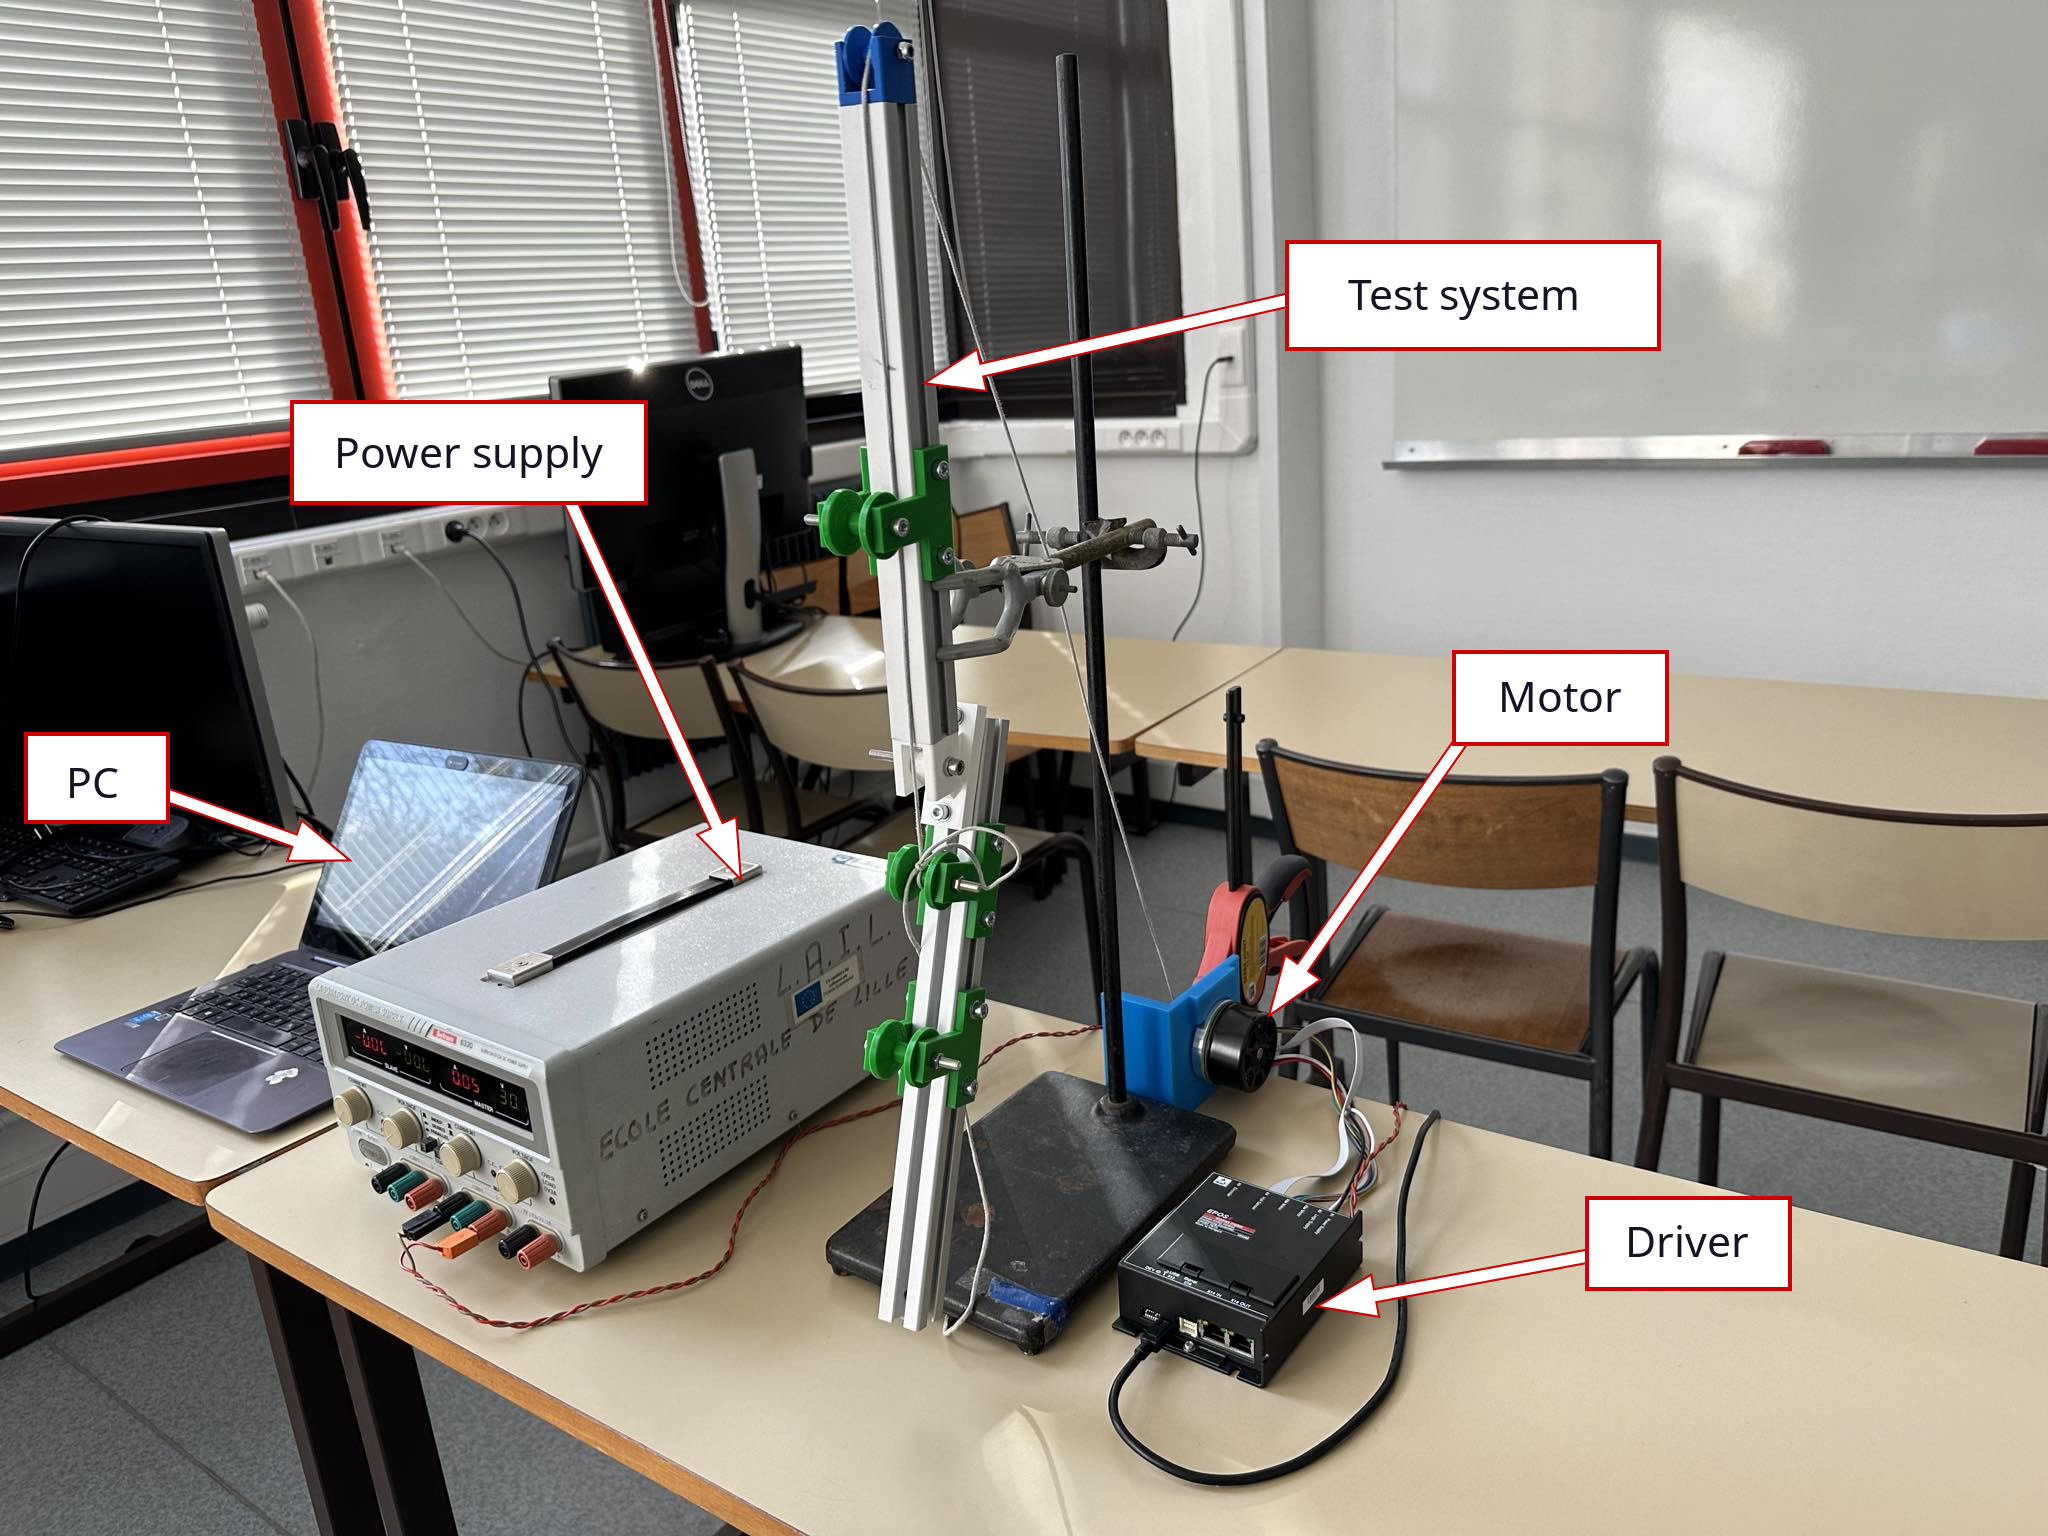
\includegraphics[width=0.8\textwidth]{setup.png}
  \caption{Experimental setup}
  \label{fig:setup}
\end{figure}
\FloatBarrier
